%% BioMed_Central_Tex_Template_v1.06
%%                                      %
%  bmc_article.tex            ver: 1.06 %
%                                       %

%%IMPORTANT: do not delete the first line of this template
%%It must be present to enable the BMC Submission system to
%%recognise this template!!

%%%%%%%%%%%%%%%%%%%%%%%%%%%%%%%%%%%%%%%%%
%%                                     %%
%%  LaTeX template for BioMed Central  %%
%%     journal article submissions     %%
%%                                     %%
%%          <8 June 2012>              %%
%%                                     %%
%%                                     %%
%%%%%%%%%%%%%%%%%%%%%%%%%%%%%%%%%%%%%%%%%


%%%%%%%%%%%%%%%%%%%%%%%%%%%%%%%%%%%%%%%%%%%%%%%%%%%%%%%%%%%%%%%%%%%%%
%%                                                                 %%
%% For instructions on how to fill out this Tex template           %%
%% document please refer to Readme.html and the instructions for   %%
%% authors page on the biomed central website                      %%
%% http://www.biomedcentral.com/info/authors/                      %%
%%                                                                 %%
%% Please do not use \input{...} to include other tex files.       %%
%% Submit your LaTeX manuscript as one .tex document.              %%
%%                                                                 %%
%% All additional figures and files should be attached             %%
%% separately and not embedded in the \TeX\ document itself.       %%
%%                                                                 %%
%% BioMed Central currently use the MikTex distribution of         %%
%% TeX for Windows) of TeX and LaTeX.  This is available from      %%
%% http://www.miktex.org                                           %%
%%                                                                 %%
%%%%%%%%%%%%%%%%%%%%%%%%%%%%%%%%%%%%%%%%%%%%%%%%%%%%%%%%%%%%%%%%%%%%%

%%% additional documentclass options:
%  [doublespacing]
%  [linenumbers]   - put the line numbers on margins

%%% loading packages, author definitions

\documentclass[twocolumn]{bmcart}% uncomment this for twocolumn layout and comment line below
%\documentclass{bmcart}

%%% Load packages
\usepackage{amsthm,amsmath}
\usepackage{siunitx}
\usepackage{mfirstuc}
%\RequirePackage{natbib}
\usepackage[colorinlistoftodos]{todonotes}
\RequirePackage{hyperref}
\usepackage[utf8]{inputenc} %unicode support
%\usepackage[applemac]{inputenc} %applemac support if unicode package fails
%\usepackage[latin1]{inputenc} %UNIX support if unicode package fails
\usepackage[htt]{hyphenat}

\usepackage{array}
\newcolumntype{L}[1]{>{\raggedright\let\newline\\\arraybackslash\hspace{0pt}}p{#1}}

%%%%%%%%%%%%%%%%%%%%%%%%%%%%%%%%%%%%%%%%%%%%%%%%%
%%                                             %%
%%  If you wish to display your graphics for   %%
%%  your own use using includegraphic or       %%
%%  includegraphics, then comment out the      %%
%%  following two lines of code.               %%
%%  NB: These line *must* be included when     %%
%%  submitting to BMC.                         %%
%%  All figure files must be submitted as      %%
%%  separate graphics through the BMC          %%
%%  submission process, not included in the    %%
%%  submitted article.                         %%
%%                                             %%
%%%%%%%%%%%%%%%%%%%%%%%%%%%%%%%%%%%%%%%%%%%%%%%%%


%\def\includegraphic{}
%\def\includegraphics{}

%%% Put your definitions there:
\startlocaldefs
\endlocaldefs


%%% Begin ...
\begin{document}

%%% Start of article front matter
\begin{frontmatter}

\begin{fmbox}
\dochead{Report from 2015 Brainhack Montreal}

%%%%%%%%%%%%%%%%%%%%%%%%%%%%%%%%%%%%%%%%%%%%%%
%%                                          %%
%% Enter the title of your article here     %%
%%                                          %%
%%%%%%%%%%%%%%%%%%%%%%%%%%%%%%%%%%%%%%%%%%%%%%

\title{Automatic Extraction of Academic Collaborations in Neuroimaging}
\vskip2ex
\projectURL{Project URL: \url{http://github.com/sderygithub/clubs-of-science}}

\author[
addressref={aff1},
corref={aff1},
email={sebastien.dery@mail.mcgill.ca}
]{\inits{SD} \fnm{Sebastien} \snm{Dery}}

%%%%%%%%%%%%%%%%%%%%%%%%%%%%%%%%%%%%%%%%%%%%%%
%%                                          %%
%% Enter the authors' addresses here        %%
%%                                          %%
%% Repeat \address commands as much as      %%
%% required.                                %%
%%                                          %%
%%%%%%%%%%%%%%%%%%%%%%%%%%%%%%%%%%%%%%%%%%%%%%

\address[id=aff1]{%
  \orgname{Montreal Neurological Institute, McGill University},
  \city{Montreal},
  \street{3801 University Street},
  \postcode{H3A 2B4},
  \postcode{QC},
  \cny{Canada}
}

%%%%%%%%%%%%%%%%%%%%%%%%%%%%%%%%%%%%%%%%%%%%%%
%%                                          %%
%% Enter short notes here                   %%
%%                                          %%
%% Short notes will be after addresses      %%
%% on first page.                           %%
%%                                          %%
%%%%%%%%%%%%%%%%%%%%%%%%%%%%%%%%%%%%%%%%%%%%%%

\begin{artnotes}
\end{artnotes}

%\end{fmbox}% comment this for two column layout

%%%%%%%%%%%%%%%%%%%%%%%%%%%%%%%%%%%%%%%%%%%%%%
%%                                          %%
%% The Abstract begins here                 %%
%%                                          %%
%% Please refer to the Instructions for     %%
%% authors on http://www.biomedcentral.com  %%
%% and include the section headings         %%
%% accordingly for your article type.       %%
%%                                          %%
%%%%%%%%%%%%%%%%%%%%%%%%%%%%%%%%%%%%%%%%%%%%%%

%\begin{abstractbox}

%\begin{abstract} % abstract
	
%Blank Abstract

%\end{abstract}



%%%%%%%%%%%%%%%%%%%%%%%%%%%%%%%%%%%%%%%%%%%%%%
%%                                          %%
%% The keywords begin here                  %%
%%                                          %%
%% Put each keyword in separate \kwd{}.     %%
%%                                          %%
%%%%%%%%%%%%%%%%%%%%%%%%%%%%%%%%%%%%%%%%%%%%%%

%\vskip1ex

%\projectURL{\url{http://github.com/sderygithub/clubs-of-science}}
%\projectURL{http://github.com/sderygithub/clubs-of-science}

% MSC classifications codes, if any
%\begin{keyword}[class=AMS]
%\kwd[Primary ]{}
%\kwd{}
%\kwd[; secondary ]{}
%\end{keyword}

%\end{abstractbox}
%
\end{fmbox}% uncomment this for twcolumn layout

\end{frontmatter}

%{\sffamily\bfseries\fontsize{10}{12}\selectfont Project URL: \url{http://github.com/sderygithub/clubs-of-science}}

%%% Import the body from pandoc formatted text
\section{Introduction}\label{introduction}

Our ability to quantitatively study large-scale social and behavioral
phenomena such as peer influence and confirmation bias within scientific
circles rest on quality and relevant data
\cite{BiologicalNetworks:Freeman2004}. Yet the compilation of specific
coauthorship databases are often restricted to certain well-defined
fields of study or publication resources, limiting the extent and depth
by which investigations can be performed. Ultimately, we aim to
understand how the social construct and its underlying dynamics
influence the trajectories of scientific endeavors
\cite{Sarigol2014:PredictingSuccess}. This work is motivated by an
interest in observing social patterns, monitoring their evolution, and
possibly understanding the emergence and spreading of ideas and their
biases in the neuroimaging community; central themes to deciphering
facts from opinions. However, before being able to fully investigate and
address these fundamental and inherently complex questions, we need to
address the extraction and validation of data. The goal of this project
was to leverage publicly available information on Google Scholar (GS) to
automatically extract coauthorship networks.

\section{Approach}\label{approach}

The tool can be accessed through a public website at
(http://cos.dery.xyz). The site is constructed using a set of openly
accessible libraries allowing the display of coauthorship networks as
interactive graphs \cite{Holten2009:ForceDirected}. Visitors can peruse
a set of pre-computed networks extracted using custom Python scripts
designed to crawl GS based on a set of predefined constraints
(e.g.~search topic, publication journal). The proposed interface offers
seamless manipulation to keep interaction straightforward and easy to
use. The simplicity of the design aims to reach a maximum number of
users, assuming a minimal level of technical knowledge.

\subparagraph{\texorpdfstring{\texttt{GraphConstruction}:}{:}}\label{section}

Scholarly citations are commonly found in standardized format,
suggesting the structure can be reliably used within an automatic
procedure. Moreover, while the result of typical search engines are not
structured towards data mining (i.e.~mixture of natural language
embedded in semi-structured tags and page links), particular
combinations of HTML tags and CSS identifiers can be leveraged to
extract specific information. This simple scheme allows the
reconstruction of large-scale networks of collaborations. Interestingly,
Google Scholar also hosts individual pages for authors' rich with
pre-computed metrics of scientific productivity and impact
(e.g.~cumulative number of citations, h-index, i10-index). This data can
be further exploited to structure and highlight part of the network.

\subparagraph{\texorpdfstring{\texttt{CommunityDetection}:}{:}}\label{section-1}

Scientific communities were detected using a greedy agglomerative
modularity optimization process \cite{Blondel08fastunfolding}.

\begin{table*}[t!]
\centering
\caption{\label{stattable}Completeness study: accuracy between the faculty roster of five major neuroimaging institutes and the neuroimaging network.}
\begin{tabular}{rccccc}
\hline
\multicolumn{1}{c}{\textbf{Institute}} & \textbf{\begin{tabular}[c]{@{}c@{}}Total Count\end{tabular}} & \textbf{Recovered} & \textbf{\begin{tabular}[c]{@{}c@{}}On Google Scholar\end{tabular}} & \textbf{Accuracy} & \textbf{\begin{tabular}[c]{@{}c@{}}Corrected Accuracy\end{tabular}} \\ \hline
\begin{tabular}[c]{@{}r@{}}McConnell Brain Imaging Center\\ (Montreal Neurological Institute)\end{tabular} & 12 & 7 & 9 & 58.33\% & 77.77\% \\
\begin{tabular}[c]{@{}r@{}}Martinos Center for Biomedical Imaging\\ (Harvard University)\end{tabular} & 39 & 12 & 22 & 30.76\% & 54.54\% \\
\begin{tabular}[c]{@{}r@{}}Cognitive-Neuroimaging Unit\\ (INSERM-CEA, France)\end{tabular} & 15 & 7 & 8 & 46.66\% & 87.50\% \\
\begin{tabular}[c]{@{}r@{}}Wellcome Trust Center for Neuroimaging\\ (University College London)\end{tabular} & 16 & 10 & 11 & 62.50\% & 90.90\% \\
\begin{tabular}[c]{@{}r@{}}FMRIB\\ (Oxford University)\end{tabular} & 17 & 8 & 11 & 47.05\% & 72.72\% \\ \hline
Totals & 99 & 44 & 61 & 49.06\% & 76.69\% \\ \hline
\end{tabular}
\end{table*}

\subparagraph{Validation:}\label{validation}

To assess the recovered network's reliability we performed a spot check
on its content. First we examined the accuracy of 100 randomly selected
researchers from the network and sought after their departmental
affiliation and publication journals to confirm their belonging to the
broad field of neuroimaging. The dependence on profiles availability
injects a strong negative bias. To better appreciate the crawling
ability to construct network we further compare with the number of
members having a Google Scholar page in the form of a corrected
accuracy.

\section{Results}\label{results}

96 researchers were confirmed to have direct institutional affiliation
to neuroscience, psychology, or biomedical engineering departments. The
remaining 4 randomly selected researchers were found to work in the
fields of human genome sequencing, image analysis, nano particles, and
pharmacology. Note that these individuals were located on the outskirts
of the main graph. To further assess completeness of the network, we
compared results with faculty rosters of 5 major neuroimaging institutes
(Table 1).

\begin{figure}[h!]
  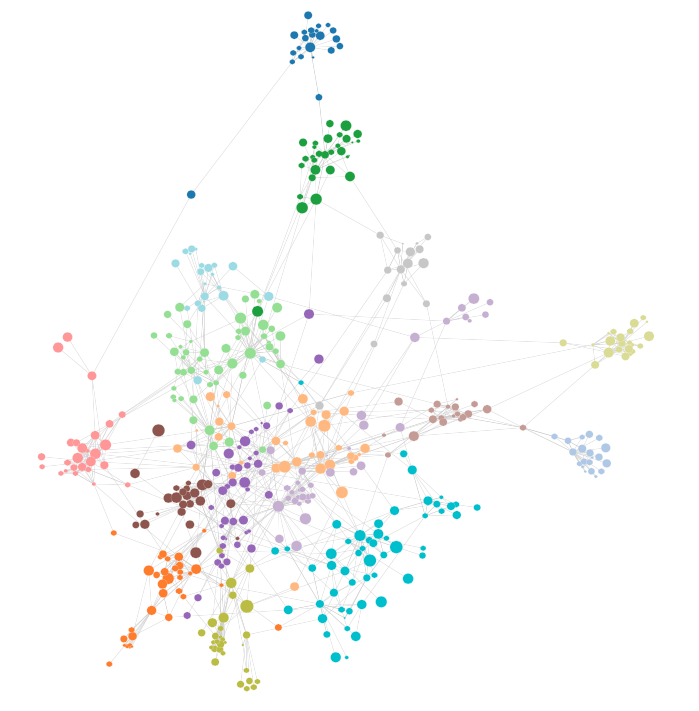
\includegraphics[width=.47\textwidth]{neuroimaging-500}
  \caption{\label{centfig}
  Coauthorship network for the field of neuroimaging. Each disk represent a single researcher with its radius encoding log10(Nc), where Nc is the number of citations. Edges stand for a binary relation of coauthorship between two researchers.}
\end{figure}

\section{Conclusions}\label{conclusions}

Accuracy results suggest a sufficient number of individuals are
registered through GS to make it a useful platform of discovery.
Meticulous inspection of the grouping suggest that communities typically
embed either a geographical or a topical component, that is to say,
certain communities are seemingly brought together by either proximity
or similarity of interest. With the increasing complexity of science,
finding accurate and relevant information on specific topics is a
challenging task. We feel that a better appreciation of the wealth and
variety of opinions within scientific communities may help enforcing the
notion that grand claims require grand evidence.

%%%%%%%%%%%%%%%%%%%%%%%%%%%%%%%%%%%%%%%%%%%%%%
%%                                          %%
%% Backmatter begins here                   %%
%%                                          %%
%%%%%%%%%%%%%%%%%%%%%%%%%%%%%%%%%%%%%%%%%%%%%%

\begin{backmatter}

\section*{Availability of Supporting Data}
More information about this project can be found at: \url{http://github.com/sderygithub/clubs-of-science}. Further data and files supporting this project are hosted in the \emph{GigaScience} repository REFXXX.

\section*{Competing interests}
None

\section*{Author's contributions}
SD wrote the software, performed tests, and wrote the report.

\section*{Acknowledgements}
The authors would like to thank the organizers and attendees of
Brainhack Montreal.

  
  
%%%%%%%%%%%%%%%%%%%%%%%%%%%%%%%%%%%%%%%%%%%%%%%%%%%%%%%%%%%%%
%%                  The Bibliography                       %%
%%                                                         %%
%%  Bmc_mathpys.bst  will be used to                       %%
%%  create a .BBL file for submission.                     %%
%%  After submission of the .TEX file,                     %%
%%  you will be prompted to submit your .BBL file.         %%
%%                                                         %%
%%                                                         %%
%%  Note that the displayed Bibliography will not          %%
%%  necessarily be rendered by Latex exactly as specified  %%
%%  in the online Instructions for Authors.                %%
%%                                                         %%
%%%%%%%%%%%%%%%%%%%%%%%%%%%%%%%%%%%%%%%%%%%%%%%%%%%%%%%%%%%%%

% if your bibliography is in bibtex format, use those commands:
\bibliographystyle{bmc-mathphys} % Style BST file
\bibliography{brainhack-report} % Bibliography file (usually '*.bib' )

\end{backmatter}
\end{document}
